\documentclass[crop,tikz,pgf]{standalone}

\usetikzlibrary{arrows,automata}

\begin{document}
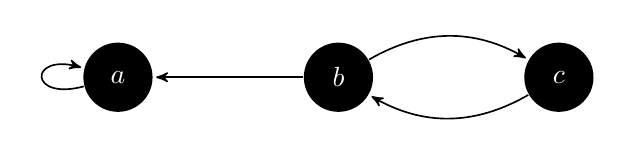
\begin{tikzpicture}[->,>=stealth',shorten >=1pt,auto,node distance=2.8cm,semithick]
	\tikzstyle{every state}=[fill=black,draw=none,text=white]

	\node[state] (A) {$a$};
	\node[state] (B) [right of=A] {$b$};
	\node[state] (C) [right of=B] {$c$};

	\path (A) [loop left] edge (A);
        \path (B) edge (A);
        \path (B) [bend left] edge (C);
	\path (C) [bend left] edge (B);
\end{tikzpicture}
\end{document}